% Settings for arara
% https://github.com/islandoftex/arara
%!TEX encoding = UTF-8 Unicode
% arara: xelatex
% arara: biber
% arara: xelatex

\documentclass[11pt]{article}
\usepackage[letterpaper, margin=1in]{geometry}

\usepackage{outlines}
\usepackage{enumitem}

%%%%%%%%%%%%%%%%%%%%%%%%%%%%%%
% Bibliography
\usepackage[style=numeric-comp, backend=biber, sorting=none, sortcites=true]{biblatex}
\addbibresource{bibliography.bib}
%%%%%%%%%%%%%%%%%%%%%%%%%%%%%%

%%%%%%%%%%%%%%%%%%%%%%%%%%%%%%
% Font
% serif fonts are more legible
\usepackage{libertine} % resembles an elegant Times New Roman
% \usepackage[sfdefault]{roboto} %sans-serif font option 
%%%%%%%%%%%%%%%%%%%%%%%%%%%%%%


%%%%%%%%%%%%%%%%%%%%%%%%%%%%%%
% Comments
\usepackage{todonotes}
\newcounter{mycomment}
 % indicate who is making a todo comment using this command
\newcommand{\mycomment}[2][]{
    \refstepcounter{mycomment}
    {\todo[inline, color={red!100!green!33},size=\small]{\textbf{[\uppercase{#1}\themycomment]:}#2}}}
%%%%%%%%%%%%%%%%%%%%%%%%%%%%%%

%%%%%%%%%%%%%%%%%%%%%%%%%%%%%%
% SI units
\usepackage{siunitx}
\DeclareSIUnit\molar{\textsc{M}}
\newcommand{\ul}[1]{\SI{#1}{\micro\liter}}
\newcommand{\ml}[1]{\SI{#1}{\milli\liter}}

\newcommand{\angs}[1]{\SI{#1}{\angstrom}}
\newcommand{\angstrom}{\textup{\AA}}
\newcommand{\um}[1]{\SI{#1}{\micro\meter}}

\newcommand{\degC}[1]{\SI{#1}{\celsius}}

\newcommand{\nanog}[1]{\si{#1}{\nano\gram}} %\ng is taken by an internal command
\newcommand{\ug}[1]{\si{#1}{\micro\gram}} %\ng is taken by an internal command
%%%%%%%%%%%%%%%%%%%%%%%%%%%%%%

%%%%%%%%%%%%%%%%%%%%%%%%%%%%%%
% Line spacing and line numbering
\usepackage{setspace}
\onehalfspacing

%% The lineno packages adds line numbers. Start line numbering with
%% \begin{linenumbers}, end it with \end{linenumbers}. Or switch it on
%% for the whole article with 
%% [modulo] numbers every five lines; see doc for arbitrary numbering
\usepackage[modulo]{lineno}
%%%%%%%%%%%%%%%%%%%%%%%%%%%%%%

\usepackage{booktabs}
\usepackage{amsmath}
\usepackage{nicematrix}

\usepackage{longtable} %format tables across multiple pages
\usepackage{booktabs} %nice looking tables

%%%%%%%%%%%%%%%%%%%%%%%%%%%%%%
% for chemical formulae
\usepackage{chemformula}
%%%%%%%%%%%%%%%%%%%%%%%%%%%%%%


% Keywords command
\newcommand{\keywords}[1]
{
  \small	
  \textbf{\textit{Keywords: }} #1
}

%%%%%%%%%%%%%%%%%%%%%%%%%%%%%%
% Manuscript title and author affiliations
\usepackage{authblk} %author block for adding affiliations easily
\setcounter{Maxaffil}{0} % allow any number of affiliations per author
\renewcommand\Affilfont{\itshape\small} % reduce affiliation font size

\title{Manuscript Title}
\author[1, *]{Jane Doe}
\author[1]{John Doe}
\author[1,2,*]{Ilya J. Finkelstein}
\affil[1]{Department of Molecular Biosciences, University of Texas at Austin, Austin, TX, 78712, USA}
\affil[2]{Center for Systems and Synthetic Biology, University of Texas at Austin, Austin, TX, 78712, USA}
\affil[*]{Correspndence: janedoe@utexas.edu; ilya@finkelsteinlab.org}

\date{}  % remove today's date from the title


%%%%%%%%%%%%%%%%%%%%%%%%%%%%%%
\begin{document}

% comment this out to remove list of todos
\listoftodos 

\maketitle
% \linenumbers % uncomment to add line numbers
\begin{abstract} 
\noindent
Aliquam erat volutpat.  Nunc eleifend leo vitae magna.  In id erat non orci commodo lobortis.  Proin neque massa, cursus ut, gravida ut, lobortis eget, lacus.  Sed diam.  Praesent fermentum tempor tellus.  Nullam tempus.  Mauris ac felis vel velit tristique imperdiet.  Donec at pede.  Etiam vel neque nec dui dignissim bibendum.  Vivamus id enim.  Phasellus neque orci, porta a, aliquet quis, semper a, massa.  Phasellus purus.  Pellentesque tristique imperdiet tortor.  Nam euismod tellus id erat.
\end{abstract}

  %% keywords here
\begin{keywords}
keyword1, keyword2, keyword3, etc.
\end{keywords}

\newpage           
\section*{Introduction}
Nullam eu ante vel est convallis dignissim.  Fusce suscipit, wisi nec facilisis facilisis, est dui fermentum leo, quis tempor ligula erat quis odio.  Nunc porta vulputate tellus.  Nunc rutrum turpis sed pede.  Sed bibendum.  Aliquam posuere.  Nunc aliquet, augue nec adipiscing interdum, lacus tellus malesuada massa, quis varius mi purus non odio.  Pellentesque condimentum, magna ut suscipit hendrerit, ipsum augue ornare nulla, non luctus diam neque sit amet urna.  Curabitur vulputate vestibulum lorem.  Fusce sagittis, libero non molestie mollis, magna orci ultrices dolor, at vulputate neque nulla lacinia eros.  Sed id ligula quis est convallis tempor.  Curabitur lacinia pulvinar nibh.  Nam a sapien \cite{lee_2022_creating}.

Aliquam erat volutpat.  Nunc eleifend leo vitae magna.  In id erat non orci commodo lobortis \cite{lee_2022_creating,dyda_2015_mechanism}.  Proin neque massa, cursus ut, gravida ut, lobortis eget, lacus.  Sed diam.  Praesent fermentum tempor tellus.  Nullam tempus.  Mauris ac felis vel velit tristique imperdiet.  Donec at pede.  Etiam vel neque nec dui dignissim bibendum.  Vivamus id enim.  Phasellus neque orci, porta a, aliquet quis, semper a, massa.  Phasellus purus.  Pellentesque tristique imperdiet tortor.  Nam euismod tellus id erat.

Pellentesque dapibus suscipit ligula.  Donec posuere augue in quam.  Etiam vel tortor sodales tellus ultricies commodo.  Suspendisse potenti.  Aenean in sem ac leo mollis blandit.  Donec neque quam, dignissim in, mollis nec, sagittis eu, wisi.  Phasellus lacus.  Etiam laoreet quam sed arcu.  Phasellus at dui in ligula mollis ultricies.  Integer placerat tristique nisl.  Praesent augue.  Fusce commodo.  Vestibulum convallis, lorem a tempus semper, dui dui euismod elit, vitae placerat urna tortor vitae lacus.  Nullam libero mauris, consequat quis, varius et, dictum id, arcu.  Mauris mollis tincidunt felis.  Aliquam feugiat tellus ut neque.  Nulla facilisis, risus a rhoncus fermentum, tellus tellus lacinia purus, et dictum nunc justo sit amet elit.


%%% Local Variables:
%%% mode: latex
%%% TeX-engine: xetex
%%% TeX-master: "main"
%%% reftex-default-bibliography: ("bibliography.bib")
%%% End:

\section*{Results}
\subsection*{First result}
Nullam eu ante vel est convallis dignissim.  Fusce suscipit, wisi nec facilisis facilisis, est dui fermentum leo, quis tempor ligula erat quis odio.  Nunc porta vulputate tellus.  Nunc rutrum turpis sed pede.  Sed bibendum.  Aliquam posuere.  Nunc aliquet, augue nec adipiscing interdum, lacus tellus malesuada massa, quis varius mi purus non odio.  Pellentesque condimentum, magna ut suscipit hendrerit, ipsum augue ornare nulla, non luctus diam neque sit amet urna.  Curabitur vulputate vestibulum lorem.  Fusce sagittis, libero non molestie mollis, magna orci ultrices dolor, at vulputate neque nulla lacinia eros.  Sed id ligula quis est convallis tempor.  Curabitur lacinia pulvinar nibh.  Nam a sapien.

\subsection*{Second result}
Lorem ipsum dolor sit amet, consectetuer adipiscing elit.  Donec hendrerit tempor tellus.  Donec pretium posuere tellus.  Proin quam nisl, tincidunt et, mattis eget, convallis nec, purus.  Cum sociis natoque penatibus et magnis dis parturient montes, nascetur ridiculus mus.  Nulla posuere.  Donec vitae dolor.  Nullam tristique diam non turpis.  Cras placerat accumsan nulla.  Nullam rutrum.  Nam vestibulum accumsan nisl.

%%% Local Variables:
%%% TeX-engine: xetex
%%% mode: latex
%%% TeX-master: "main"
%%% reftex-default-bibliography: ("bibliography.bib")
%%% End:

\section*{Discussion}

\mycomment[IJF]{Sample comment about a discussion point}

%%% Local Variables:
%%% mode: latex
%%% TeX-master: "main"
%%% TeX-engine: xetex
%%% reftex-default-bibliography: ("bibliography.bib")
%%% End:

\section*{Materials and Methods}
\subsection*{Proteins and nucleic acids} 
Nullam eu ante vel est convallis dignissim.  Fusce suscipit, wisi nec facilisis facilisis, est dui fermentum leo, quis tempor ligula erat quis odio.  Nunc porta vulputate tellus.  Nunc rutrum turpis sed pede.  Sed bibendum.  Aliquam posuere.  Nunc aliquet, augue nec adipiscing interdum, lacus tellus malesuada massa, quis varius mi purus non odio.  Pellentesque condimentum, magna ut suscipit hendrerit, ipsum augue ornare nulla, non luctus diam neque sit amet urna.  Curabitur vulputate vestibulum lorem.  Fusce sagittis, libero non molestie mollis, magna orci ultrices dolor, at vulputate neque nulla lacinia eros.  Sed id ligula quis est convallis tempor.  Curabitur lacinia pulvinar nibh.  Nam a sapien.


\subsection*{Other sub-section }
\subsubsection*{Sub-sub-section example}
Lorem ipsum dolor sit amet, consectetuer adipiscing elit.  Donec hendrerit tempor tellus.  Donec pretium posuere tellus.  Proin quam nisl, tincidunt et, mattis eget, convallis nec, purus.  Cum sociis natoque penatibus et magnis dis parturient montes, nascetur ridiculus mus.  Nulla posuere.  Donec vitae dolor.  Nullam tristique diam non turpis.  Cras placerat accumsan nulla.  Nullam rutrum.  Nam vestibulum accumsan nisl.

%%% Local Variables:
%%% mode: latex
%%% TeX-master: "main"
%%% End:

\section*{Supplemental Information}

Supplemental information includes zzz figures and zzz tables. 
% Github repo? Nucleotide sequence deposition? Any other databases or resources?

\section*{Declarations}

\paragraph{Author Contributions}

zzz, zzz. and I.J.F. conceived the project. zzz and zzz performed all
experiments and analyzed the data. zzz and zzz prepared the figures. I.J.F.
secured the funding. I.J.F. supervised the project. zzz and zzz and I.J.F. wrote the manuscript with input from all co-authors.

\paragraph{Funding}

This work was supported by NIGMS grants zzz (to I.J.F.), the Welch Foundation grant F-1808 (to I.J.F.), and the College of Natural Sciences Catalyst Award for seed funding. 

\paragraph{Declaration of Interests}
zzz and I.J.F. have filed a patent application relating to zzz. 

%%% Local Variables:
%%% mode: latex
%%% TeX-master: "main"
%%% reftex-default-bibliography: ("bibliography.bib")
%%% End:


\newpage 
          
\printbibliography

%%%%%%%%%%%%%%%%%%%%%%%%%%%%%%%%%%%%%%%%%%%%%%%%%%%%%%%%%%%%%%%%%%%%%
% Figures
%%%%%%%%%%%%%%%%%%%%%%%%%%%%%%%%%%%%%%%%%%%%%%%%%%%%%%%%%%%%%%%%%%%%%

\newpage

%%%%%%%%%%%%% Figure 1
\begin{figure}
\centering
\begin{subcaptiongroup}
\phantomcaption\label{fig:1A} % add one of these for each subpanel
\phantomcaption\label{fig:1B} % add one of these for each subpanel
\end{subcaptiongroup}
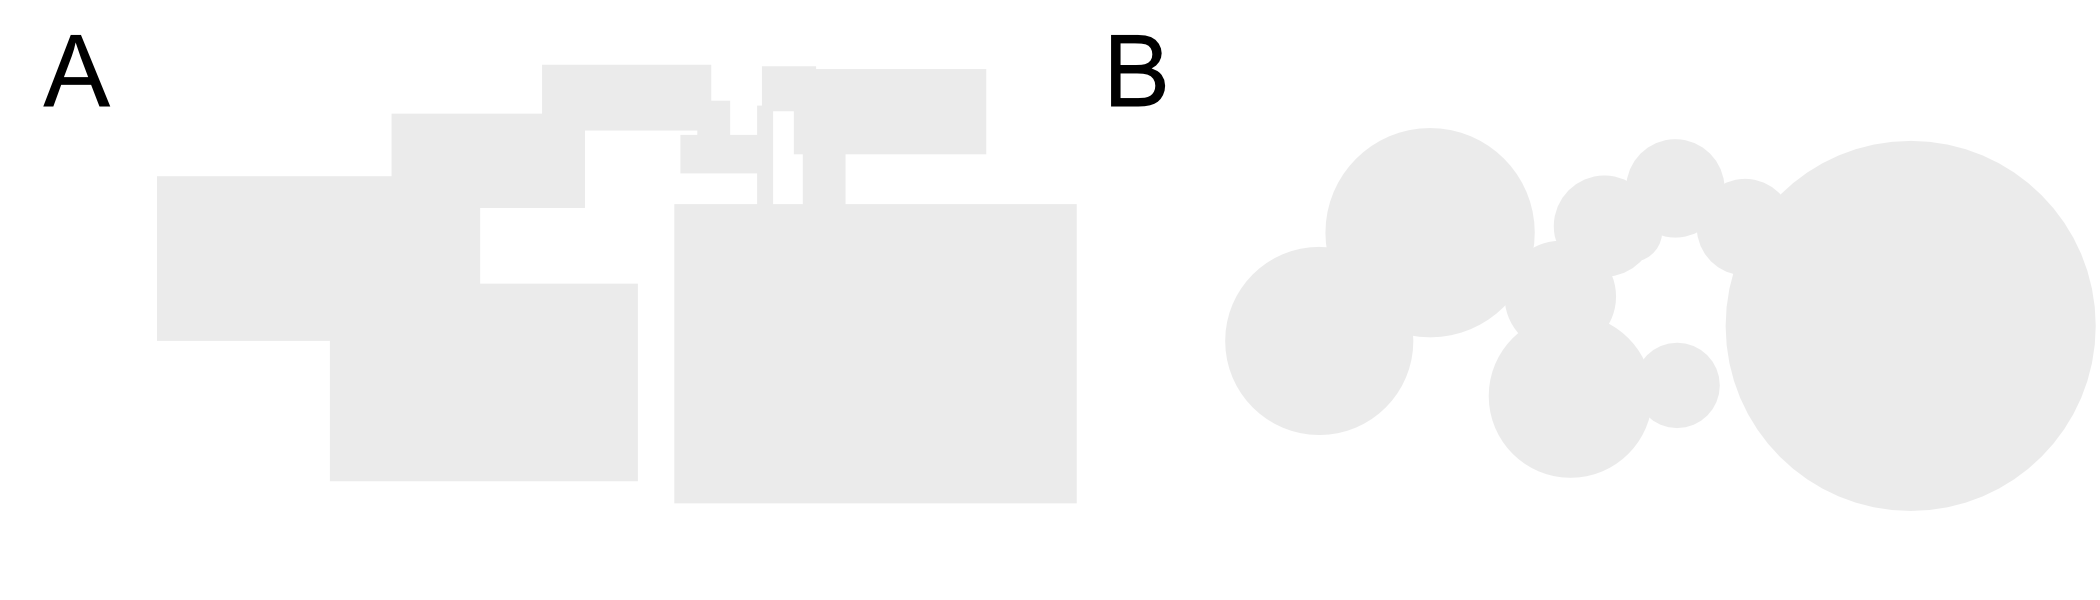
\includegraphics[width=1\textwidth]{figures/sampfig.png}
\caption{\textcolor{Highlight}{\textbf{Schematic illustrations of apparatus design.}}\\
(A)
Some text.\\
(B)
More text.\\
(C) 
Last text.
}
\label{fig:F1}

\end{figure}

%%%%%%%%%%%%%%%%%%%%%%%%%%%%%%%%%%%%%%%%%%%%%%%%%%%%%%%%%%%%%%%%%%%%%
% SUPPLEMENTAL Figures
%%%%%%%%%%%%%%%%%%%%%%%%%%%%%%%%%%%%%%%%%%%%%%%%%%%%%%%%%%%%%%%%%%%%%

\beginsupplement % <- renumbers everything and starts figure naming with "S" per local.sty
\end{document}

% Settings for Emacs
%%% Local Variables:
%%% TeX-engine: xetex
%%% mode: latex
%%% TeX-master: t
%%% End:


